\Chapter{Tervezés}

A koncepciók, továbbá a felhasznált technológia kidolgozása után magára az alkalmazás tervezésére fordult a figyelmem. Elsőként kidolgoztam, hogy az alkalmazás kezelése hogyan menjen végbe, hogyan lehetne felhasználóbaráttá, ám mégis univerzálissá (a jövőbeli könnyebb fejlesztés jegyében) és könnyeddé alakítani az alkalmazást. Végül amellett döntöttem, hogy egy paranccsor alapú interaktív alkalmazást fogok létrehozni, amely paranccsori argumentumok nélkül fog működni.

\Section{Felhasználói felület, use-case diagram, use-case leírások}

Maga a tervezett felhasználói felület több menüpontból áll. Legelőször a főmenübe jutunk, ahonnan tudunk választani az alapfunkcionalitások közül, amelyeket már az előző, Koncepció című fejezetben megemlítettem. Ezek a szervereket jelentik, továbbá az iptables tűzfalat. Ezeken belül is többféle menüpontok találhatóak meg a kiválasztott funkcionalitásnak megfelelően. A menüpontok végén mindegyik almenü esetén szerepel a Visszalépés lehetőség. A navigálás egyszerűsítése érdekében minden egyes menüpontnak külön számot kell tartalmaznia. Menü váltáshoz az adott menüpont azonosító számát kell beírnunk, és ENTER-t kell nyomnunk. Néhány menüpont akár különböző adatokat is kérhet be, például weboldal létrehozásakor a weboldal címét, domainjét.
A program use-case diagramja \myaref{fig:usecase_diagram} ábrán található.

\begin{figure}[!h]
\centering
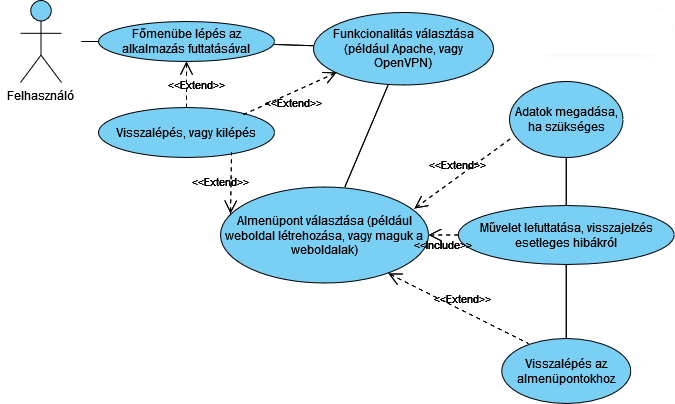
\includegraphics[scale=0.42]{images/usecase_diagram.png}
\caption{A program use-case diagramja}
\label{fig:usecase_diagram}
\end{figure}

\pagebreak

\SubSection{OpenVPN use-case leírása}

Az OpenVPN szerver konfigurálása közben a következőekben bemutatott esetek valósulhatnak meg. 

Ha nincs még feltelepítve az openvpn csomag, akkor fel kell telepítenünk azt. A csomag telepítése az \textit{apt-get} segédprogrammal megvalósítható, a csomag megléte pedig a \textit{dpkg-query} paranccsal ellenőrizhető, amellyel lekérhető egy adott csomag állapota megfelelő paraméterezéssel.

Feltelepítés után több dolgot is elő kell készíteni:
\begin{itemize}
	\item fel kell telepíteni az Easy-RSA-t, hogy saját tanusítványkezelőnk legyen mind a szerver mind a kliensek számára,
	\item létre kell hozni az Easy-RSA segítségével egy központi tanusítványt, továbbá a szervernek is egy tanusítványt és privát kulcsot,
	\item létre kell hozni az OpenVPN szervernek az \textit{\detokenize{/etc/openvpn}} adott aljegyzékében egy felhasználót \textit{\detokenize{/bin/false}} shellel a megnövelt biztonságért, amelyben futhat; ha már létezik ráfrissítünk, hogy biztos jó beállításai legyenek,
	\item létre kell hozni egy üres crl.pem fájlt, melybe később a visszavont kliensek tanusítványai kerülnek,
	\item generálni kell tls-auth fájlt az \textit{\detokenize{openvpn --genkey tls-auth}} parancs segítségével,
	\item be kell konfigurálni magát a szervert a \textit{server.conf}-ban: meg kell adni a létrehozott fájlok pathját az adott paraméterekhez (crl-verify, ca, cert, key, askpass, tls-crypt), meg kell adni a usert a server daemon számára (user, group), továbbá meg kell adni a chroot elérési útvonalát, amely a felhasználó home directoryja lesz,
	\item be kell állítani a \textit{\detokenize{/etc/default/openvpn}} fájlban az AUTOSTART értéket all-ra, és frissíteni kell a systemctl daemon-nal kapcsolatos beállításait a \textit{systemctl daemon-reload} paranccsal,
	\item be kell állítani a megfelelő jogosultságokat (chown és chmod) a fájlokon, jegyzékeken,
	\item ezek után pedig újra kell indítanunk a szervert.
\end{itemize}

Az előkészületek után lehet új kliens tanusítványt és privát kulcsot létrehozni, ezt a \textit{build-client-full} paraméterrel lehet megtenni az EasyRSA-ban. Célszerű jelszót használni a kulcs titkosításához. Ezután pedig egy minta konfiguráció módosításával tudjuk bekonfigurálni az új kliensünk konfigurációját, amelyet használhat az OpenVPN client segítségével. Ha valamely kliens hozzáférést vissza szeretnénk vonni, a \textit{revoke} EasyRSA paraméter van a segítségünkre. Ezután le kell futtatni a \textit{gen-crl} parancsot is, hogy tudja az OpenVPN szerver, mely kliens tanusítványok lettek visszavonva. A kliensek listája az EasyRSA mappájában az index.txt-ben található meg, ezt kell beolvasnunk ahhoz, hogy a jelenlegi kliensek listáját megkapjuk.

\SubSection{Apache use-case leírása}

Az Apache2 szerver adminisztrálása közben is több eset felmerülhet.

Legelőször is, ha még nincs feltelepítve az apache2 csomag, akkor azt fel kell telepítenünk. A feltelepítés és a csomag-ellenőrzés módszere megegyezik az OpenVPN esetében lévővel.

A csomag sikeres telepítése után az OpenVPN-hez képest valamivel kevesebb dolgot kell előkészítenünk:
\begin{itemize}
	\item létre kell hozni egy felhasználót \textit{\detokenize{/bin/false}} shellel, amelyben futhat maga az Apache2 daemon; ha ez már létezik, akkor beállításait frissíteni kell,
	\item létre kell hoznunk egy jegyzéket a weboldalak konfigurációinak tárolására (websiteconfigs), továbbá egy jegyzéket, ahol később a weboldalak tartalmai lesznek (wwwdatas),
	\item be kell állítani a megfelelő jogosultságokat (chown és chmod) a fájlokon, jegyzékeken,
	\item be kell konfigurálnunk a szervert úgy, hogy betöltse a saját weboldalunk konfigurációs fájljait (IncludeOptional beállítás); továbbá azt is be kell konfigurálnunk, hogy a wwwdatas jegyzéket elérhesse a daemon (Directory blokk létrehozása),
	\item be kell állítanunk az \textit{\detokenize{/etc/apache2/envvars}} fájlban az \detokenize{APACHE_RUN_USER, APACHE_RUN_GROUP} beállításokat, hogy a daemon az újonnan létrehozott felhasználót használja,
	\item ezek után újra kell indítanunk a szervert.
\end{itemize}
	
A megfelelő beállítások után már hozhatunk létre weboldalakat. Ehhez szükségünk lesz egy konfigurációs fájlra, amelyet a már előzőleg elkészített websiteconfigs jegyzékbe el kell helyezzünk. A konfigurációs fájlt egy megadott mintából kiindulva írjuk meg, kicserélve a megfelelő paramétereket (például ServerName, DocumentRoot). Ezután létre kell hoznunk a weboldalnak egy jegyzéket a wwwdatas jegyzéken belül, amelybe a weboldal tartalma kerül. A weboldalhoz létrehozunk egy index.html-t, amelybe egy üdvözlő üzenet kerül. Ezek után beállítjuk az újonnan létrehozott jegyzékek, fájlok jogosultságait, tulajdonosait. Weboldal törlésekor ki kell törölnünk az adott konfigurációs fájlt, a wwwdatas jegyzéken belül a weboldal jegyzékét, majd újra kell indítanunk a szervert.

SSL beállítása esetén először is meg kell győződnünk arról, hogy a headers és az ssl modul rendelkezésünkre áll, ezt a \textit{a2enmod headers} és \textit{a2enmod ssl} paranccsal tudjuk megtenni. Ezután megkeressük a Let's Encrypt által létrehozott minta SSL konfigurációt (amely frissítésre kerül általában automatikusan a megfelelő legújabb normáknak), és átmásoljuk egy megfelelő helyre. Miután sikeresen átmásoltuk, létrehozunk egy IfModule és VirtualHost blokkot (amely a 443-as portra mutat), amelyben el kell helyezni a már másik VirtualHost blokkban lévő beállításokat, továbbá ki kell egészíteni azt az SSL let's Encrypt fájl Include-olásával, paramétereivel (SSLCertificateFile, SSLCertificateKeyFile, SSLOpenSSLConfCmd, SSLCompression, Header).

\pagebreak

\SubSection{Nginx use-case leírása}

Az nginx szerver adminisztrálása hasonló lépéseket követel meg, mint az Apache2 szerver adminisztrálása.

Itt is a csomag telepítésével kezdünk, ha még nincs feltelepítve az nginx csomag. A feltelepítés és a csomag-ellenőrzés módszere megegyezik az OpenVPN esetében lévővel.

A csomag sikeres telepítése után szintén több dolgot szükséges előkészíteni:
\begin{itemize}
	\item létre kell hozni egy felhasználót \textit{\detokenize{/bin/false}} shellel, amelyben futhat maga az Apache2 daemon; ha ez már létezik, akkor beállításait frissíteni kell,
	\item létre kell hoznunk egy jegyzéket a weboldalak konfigurációinak tárolására (websiteconfigs), továbbá egy jegyzéket, ahol később a weboldalak tartalmai lesznek (wwwdatas),
	\item be kell állítani a megfelelő jogosultságokat (chown és chmod) a fájlokon, jegyzékeken,
	\item be kell konfigurálnunk a szervert úgy, hogy betöltse a saját weboldalunk konfigurációs fájljait (include beállítás), továbbá be kell állítanunk, hogy a daemon az újonnan létrehozott felhasználót használja (user paraméter).
\end{itemize}

A megfelelő beállítások után már hozhatunk létre weboldalakat. Ehhez szükségünk lesz egy konfigurációs fájlra, amelyet a már előzőleg elkészített websiteconfigs jegyzékbe el kell helyezzünk. A konfigurációs fájlt egy megadott mintából kiindulva írjuk meg, kicserélve a megfelelő paramétereket (például \detokenize{server_name, root}). Ezután létre kell hoznunk a weboldalnak egy jegyzéket a wwwdatas jegyzéken belül, amelybe a weboldal tartalma kerül. A weboldalhoz létrehozunk egy index.html-t, amelybe egy üdvözlő üzenet kerül. Ezek után beállítjuk az újonnan létrehozott jegyzékek, fájlok jogosultságait, tulajdonosait. Weboldal törlésekor ki kell törölnünk az adott konfigurációs fájlt, a wwwdatas jegyzéken belül a weboldal jegyzékét, majd újra kell indítanunk a szervert.

SSL beállítása esetén először megkeressük a Let's Encrypt által létrehozott minta SSL konfigurációt (amely frissítésre kerül általában automatikusan a megfelelő legújabb normáknak), és átmásoljuk egy megfelelő helyre. Miután sikeresen átmásoltuk, a már meglévő HTTP beállításokhoz a weboldal konfigurációjában beszúrjuk egy include beállítás segítségével. Ezután beállítjuk a megfelelő SSL paramétereket (\detokenize{add_header, ssl_dhparam, ssl_certificate, ssl_certificate_key, if ($scheme != "https") blokk, listen 443 ssl}), a már meglévő HTTP beállításokhoz való hozzáfűzéssel.

\SubSection{certbot use-case leírása}

Webszerverek üzemeltetése során szóba jöhet az SSL beállítása, ehhez lesz nekünk segítségül a certbot.

A certbot telepítése előtt a snapd csomagot szükséges telepítenünk az apt csomagkezelő segítségével, majd azt le kell frissíteni a \textit{snapd install --stable core} parancs segítségével. Ezután telepíthető a certbot a \textit{snapd install --stable --classic certbot} parancs segítségével. Hogy megtudjuk, már telepítve van-e a csomag, a \textit{snap list} parancs értelmezése van segítségünkre.

A csomag telepítése után létre kell hozni egy szimbolikus linket a \textit{ln -s /snap/bin/certbot /usr/bin/certbot} parancs segítségével, így tudjuk bárhonnan használni a certbot parancsot. SSL tanusítványok létrehozását kétféleképp is hozhatunk létre: HTTP-01 challenge és DNS-01 challenge segítségével. Mindkettőhöz külön parancs tartozik, a HTTP-01 challenge könnyebben automatizálható megfelelő paraméterekkel, a DNS-01-hez pedig szükséges egyedi authentikációs szkript létrehozása. Az SSL tanusítvány sikeres kiállítása után konfigurálnunk kell webszervereinket a már előzőleg megemlített módon. Célszerű dhparam fájlt is létrehozni, minél nagyobb bitszámmal, a megnövelt biztonság érdekében.

\SubSection{iptables use-case leírása}

Bármely szerver üzemeltetése során felmerül egy tűzfal beállítása, mint egy védelmi rendszer elemeként.

Az iptables használatához először meg kell győződnünk róla, hogy már fel van-e telepítve. Ha nincs, az apt csomagkezelő segítségével telepíteni tudjuk. Ezután beolvassuk és értelmezzük a már meglévő iptables szabályokat annak érdekében, hogy például tudjuk mely portok lehetnek nyitva, zárva. A jelenlegi iptables szabályokat a \textit{iptables-save} parancs segítségével tudjuk megnézni, ezt a fájlt szükséges értelmeznünk. A jelenlegi szabálykészletek felülírására a \textit{iptables-restore} parancsot használjuk.

Új portot az \textit{\detokenize{iptables -A INPUT -i interf}é\detokenize{sz -p protokoll --dport port --source }ipcím\detokenize{ -j ACCEPT}} parancs segítségével tudunk engedélyezni. Ebben a parancsban a source paraméter elhagyható. Ezt a szabályt célszerű legelőlre beszúrni.

Portot lezárni az \textit{\detokenize{iptables -A INPUT -i interf}é\detokenize{sz -p protokoll --dport port --source }ipcím\detokenize{ -j DROP}} parancs segítségével tudunk engedélyezni. Ebben a parancsban a source paraméter elhagyható. Ez a szabály bárhova beszúrható.

Új kimenő kapcsolatot az \textit{\detokenize{iptables -A OUTPUT -i interf}é\detokenize{sz -p protokoll --dport port --destination }ipcím\detokenize{ -j ACCEPT}} parancs segítségével tudunk engedélyezni. Ezt a szabályt célszerű legelőlre beszúrni. A protokoll és a port paraméter kihagyható.

Minden bejövő kapcsolatot, kivéve az engedélyezettet az \textit{\detokenize{iptables -A INPUT -i interf}é\detokenize{sz -j DROP}} paranccsal tudunk letiltani. Ezt a szabályt a szabályok levégére kell beszúrnunk.
Minden kimenő kapcsolatot, kivéve az engedélyezettet az \textit{\detokenize{iptables -A OUTPUT -i interf}é\detokenize{sz -j DROP}} paranccsal tudunk letiltani. Ezt a szabályt a szabályok levégére kell beszúrnunk.

Az előzőleg példaként adott parancsoknál az interfész paraméter mindenhol kihagyható (ekkor mindegyikre vonatkozni fog).

OpenVPN NAT-ot a következő parancsokkal tudunk engedélyezni:
\begin{itemize}
	\item \detokenize{iptables -A FORWARD -i IF_MAIN -o IF_TUNNEL -m state --state ESTABLISHED,RELATED -j ACCEPT}, ahol az \detokenize{IF_MAIN} a fő interfészünk, az \detokenize{IF_TUNNEL} pedig általában a tun0 interfész,
	\item \detokenize{iptables -A FORWARD -s YOUR_OPENVPN_SUBNET -o $IF_MAIN -j ACCEPT}, ahol az \detokenize{YOUR_OPENVPN_SUBNET} az OpenVPN szerverünk IP címét és subnetjét tartalmazza,
	\item \detokenize{iptables -t nat -A POSTROUTING -s YOUR_OPENVPN_SUBNET -o}\\\detokenize{IF_MAIN -j MASQUERADE}, ahol az \detokenize{YOUR_OPENVPN_SUBNET} az \\OpenVPN szerverünk IP címét és subnetjét tartalmazza, továbbá az \detokenize{IF_MAIN} a fő interfészt.
\end{itemize}

\pagebreak

A következő leírásokban, ábrákban bemutatom azokat a modulok struktúráját\\(UML diagramját), amelyek az előzőleg kifejtett use-casekat megvalósítják.

A program felépítése az OO alapelveket igyekszik követni. Elsősorban modulokból áll, amelyek osztályként is értelmezhetőek. Vannak olyan modulok, amelyekben csak a helyi scopeban elérhető kódok vagy változók vannak, tehát "private" elérésűek. Vannak olyan modulok, amelyekben több osztályok is találhatóak. A main modul (vagyis maga a main.lua) a felhasználói interfészt tartalmazza, ez használja fel a legtöbb modult.

A \myref{fig:visibilityrules} ábrán tekinthetőek meg a láthatósági szabályok az UML diagramokon.
\begin{figure}[h!]
	\centering
	\begin{tikzpicture}
		\begin {class}[text width=0.35\textwidth]{Láthatósági szabályok}{0, 0}
			\attribute {- Private}
			\attribute {+ Public}
		\end {class}
	\end {tikzpicture}
	\caption{Láthatósági szabályok az UML diagramokon}
	\label{fig:visibilityrules}
\end{figure}

\Section{general, apt\_packages, utils modulok felépítése, feladata}

Legelőször a \detokenize{general, linux, apt_packages} és az utils modul került megtervezésre. Felépítésük \myaref{fig:generalandaptpackages} ábrán látható.

\begin{figure}[h!]
	\centering
	\begin{tikzpicture}
		\begin {class}[text width=0.455\textwidth]{general}{0, 0}
			\attribute {+ \detokenize{lineEnding : string}}
			\operation {+ \detokenize{getOSType()}}
			\operation {+ \detokenize{clearScreen()}}
			\operation {+ \detokenize{sleep(n)}}
			\operation {+ \detokenize{strSplit(str, sep)}}
			\operation {+ \detokenize{deepCompare(tbl1, tbl2)}}
			\operation {+ \detokenize{concatPaths(...) -> varargs}}
			\operation {+ \detokenize{extractDirFromPath(path)}}
			\operation {+ \detokenize{readAllFileContents(filePath)}}
			\operation {+ \detokenize{trim2(s)}}
		\end {class}
		\begin {class}[text width=0.44\textwidth]{\detokenize{apt_packages}}{7.8, 0}
			\operation {+ \detokenize{isPackageInstalled(packageName)}}
			\operation {+ \detokenize{installPackage(packageName)}}
		\end {class}
	\end {tikzpicture}
	\caption{A general és \detokenize{apt_packages} modul felépítése}
	\label{fig:generalandaptpackages}
\end{figure}

A general modulban olyan funkciók és változók találhatóak, amelyek a legtöbb operációs rendszeren működnek, és fontos szerepet töltenek be a program működése közben.

Az \detokenize{apt_packages} modul Linux-specifikus kódokat tartalmaz, a modul feladata az apt program segítségével a csomagok menedzselése, telepítése.

Az utils modul legfőképp hibakeresésre volt használva, jelenleg épp nincs alkalmazva a program kódjában, így ezt a modult nem mutatom be.

\pagebreak

\Section{linux modul felépítése, feladatai}

A \myref{fig:linux_module} számú UML diagramon a linux nevezetű modult fogom bemutatni, amely linux-specifikus kódrészleteket tartalmaz. Erre a modulra épül a legtöbb modul.

\begin{figure}[h!]
\centering
	\begin{tikzpicture}%[scale=0.85, every node/.style={scale=0.85}]
		\begin {class}[text width=0.9\textwidth]{linux}{0, 0}
			\operation {+ \detokenize{exists(file)}}
			\operation {+ \detokenize{isDir(path)}}
			\operation {+ \detokenize{listDirFiles(path)}}
			\operation {+ \detokenize{mkDir(path)}}
			\operation {+ \detokenize{deleteFile(path))}}
			\operation {+ \detokenize{deleteDirectory(path)}}
			\operation {+ \detokenize{execCommand(cmd)}}
			\operation {+ \detokenize{getServiceStatus(serviceName)}}
			\operation {+ \detokenize{isServiceRunning(serviceName)}}
			\operation {+ \detokenize{isProcessRunning(name)}}
			\operation {+ \detokenize{stopService(serviceName)}}
			\operation {+ \detokenize{startService(serviceName)}}
			\operation {+ \detokenize{restartService(serviceName)}}
			\operation {+ \detokenize{systemctlDaemonReload()}}
			\operation {+ \detokenize{checkIfUserExists(userName)}}
			\operation {+ \detokenize{createUserWithName(userName, comment, shell, homeDir)}}
			\operation {+ \detokenize{updateUser(userName, comment, shell)}}
			\operation {+ \detokenize{getUserHomeDir(userName)}}
			\operation {+ \detokenize{execCommandWithProcRetCode(cmd, linesReturned, envVariables, redirectStdErrToStdIn)}}
			\operation {+ \detokenize{copy(from, to)}}
			\operation {+ \detokenize{copyAndChown(user, from, to)}}
			\operation {+ \detokenize{chown(path, userName, isDir)}}
			\operation {+ \detokenize{chmod(path, perm, isDir)}}
		\end {class}
	\end {tikzpicture}
	\caption{A linux modul felépítése}
	\label{fig:linux_module}
\end{figure}

A linux modul feladatai szerteágazóak:

\begin{itemize}
	\item vannak benne fájl- és könyvtár manipulációs funkciók,
	\item vannak benne parancsfuttató funkciók (amelyek közül az egyik tökéletesen kompatibilis Windows-sal is), továbbá servicet és systemctlt kezelő funkciók,
	\item vannak benne felhasználókat módosító funkciók (felhasználók létrehozása, módosítása, felhasználó létezésének ellenőrzése, felhasználó home dir lekérése),
	\item vannak benne fájl vagy jegyzék tulajdonost változtató funkciók,
	\item vannak benne fájl és jegyzék hozzáférési szabályokat változtató funkciók.
\end{itemize}

\Section{OpenVPN modulok felépítései, feladatai}

A következőekben az OpenVPN szerver kezelését kezdtem el megtervezni, implementálni. Az összes modul a program jegyzékén belül a \textbf{modules/vpnHandler} jegyzékben található meg.

Több részmodulra lett szétosztva:
\begin{itemize}
	\item \textbf{OpenVPN}: ez maga bootstrap modul, ebben van OpenVPN csomagot feltelepítő funkció, szervert indító/leállító funkció, továbbá ez a modul tölti be a \detokenize{server_impl} modult
	\item \textbf{\detokenize{server_impl}}: ez a modul kezeli a szerverrel kapcsolatos legtöbb dolgot:
	
	előkészíti a könyvtárakat, feltelepíti az Easy-RSA Certificate kezelőt, létrehoz egy saját tanusítványkezelőt (\textit{Certificate Authority}-t), szerver-oldali tanusítványokat és kulcsfájlokat generál, saját OpenVPN felhasználót hoz létre a szervernek, tls-auth/tls-crypt kulcsot generál, a szerver konfigurációt beüzemeli, beállítja a server daemon auto-startot a \textit{/etc/default/openvpn} fájlban

	\item \textbf{\detokenize{config_handler}}: az OpenVPN szerver és kliens konfigját kezelő modul, konfigurációs fájl beolvasást és írást valósít meg. A parser és writer az eredeti OpenVPN parser kódja alapján épült, amely megtalálható a \cite{openvpn_parser} hivatkozás alatt.
	\item \textbf{\detokenize{clienthandler_impl}}: ez a modul kezeli teljesen a klienssel kapcsolatos dolgokat:
	
	kliens tanusítványt, privát kulcsot hoz létre; kliens konfigurációt hoz létre, amelybe beleszúrja a generált fájlok tartalmát (így 1 db konfigurációs fájlra van szüksége az OpenVPN kliensnek); tanusítvány visszavonást támogat; továbbá le lehet kérni az összes jelenlegi klienst, amelyek valósak (nincsenek visszavonva)
\end{itemize}

Maga az OpenVPN bootstrap és \detokenize{config_handler} modul nagyon egyszerű felépítésű, amely látható is \myaref{fig:openvpn_module} és \myaref{fig:openvpn_config_handler_module} ábrán. 
\begin{figure}[h!]
\centering
	\begin{tikzpicture}[scale=0.83, every node/.style={scale=0.83}]
		\begin {class}[text width=0.7\textwidth]{OpenVPN}{0, 0}
			\attribute {+ \detokenize{errors : table}}
			\attribute {+ \detokenize{serverImpl -> }\textbf{OpenVPN\_server\_impl} module}
			\operation {+ \detokenize{isOpenVPNInstalled()}}
			\operation {+ \detokenize{installOpenvpn()}}
			\operation {+ \detokenize{isRunning()}}
			\operation {+ \detokenize{stopServer()}}
			\operation {+ \detokenize{startServer()}}
			\operation {+ \detokenize{initDirs()}}
		\end {class}
	\end {tikzpicture}
	\caption{Az OpenVPN bootstrap modul felépítése}
	\label{fig:openvpn_module}
\end{figure}

\begin{figure}[h!]
\centering
	\begin{tikzpicture}[scale=0.83, every node/.style={scale=0.83}]
		\begin {class}[text width=0.7\textwidth]{\detokenize{OpenVPN_config_handler}}{0, 0}
			\operation {+ \detokenize{parseOpenVPNConfig(linesInStr)}}
			\operation {+ \detokenize{writeOpenVPNConfig(parsedLines)}}
		\end {class}
	\end {tikzpicture}
	\caption{Az \detokenize{OpenVPN_config_handler} modul felépítése}
	\label{fig:openvpn_config_handler_module}
\end{figure}

A \detokenize{server_impl} modul minden OpenVPN szerverrel kapcsolatos művelet magja, ezért sok funkcióval rendelkezik. Felépítése \myaref{fig:openvpn_server_impl_module} ábrán látható. 

A klienseket kezelő \detokenize{OpenVPN_clienthandler_impl} modulban pedig két osztály is helyet foglal az OO alapelveket követve. Struktúrája \myaref{fig:openvpn_clienthandler_impl_module} ábrán látható.

\begin{figure}[h]
	\centering
	\begin{tikzpicture}[scale=0.84, every node/.style={scale=0.84}]
		\begin {class}[text width=1\textwidth]{\detokenize{OpenVPN_server_impl}}{0, 0}
			\attribute {- \detokenize{bootstrapModule -> }\textbf{\detokenize{OpenVPN}} module}
			\attribute {- \detokenize{caPass : string}}
			\attribute {- \detokenize{serverKeyPass : string}}
			\attribute {- \detokenize{sampleConfigFileContent : string}}
			\attribute {+ \detokenize{errors : table}}
			\operation {- \detokenize{registerNewError(errorName)}}
			\operation {- \detokenize{getConfigFilePath(openVPNConfigDir)}}
			\operation {+ \detokenize{constructor(_bootstrapModule)}}
			\operation {+ \detokenize{resolveErrorToStr(error)}}
			\operation {+ \detokenize{getEasyRSADir()}}
			\operation {+ \detokenize{getCAPass()}}
			\operation {+ \detokenize{getOpenVPNBaseConfigDir()}}
			\operation {+ \detokenize{isEasyRSAInstalled()}}
			\operation {+ \detokenize{formatPathInsideEasyRSAInstallCache(path)}}
			\operation {+ \detokenize{formatPathInsideBasedir(path)}}
			\operation {+ \detokenize{initDirs()}}
			\operation {+ \detokenize{installEasyRSA()}}
			\operation {+ \detokenize{getEasyRSAPKiDir()}}
			\operation {+ \detokenize{initEasyRSA()}}
			\operation {+ \detokenize{enableAllAutostartInDefault()}}
			\operation {+ \detokenize{getOpenVPNSubnet()}}
			\operation {+ \detokenize{checkServerConfig(homeDir, openVPNConfigDir)}}
			\operation {+ \detokenize{checkOpenVPNUserExistence()}}
			\operation {+ \detokenize{createOpenVPNUser(homeDir)}}
			\operation {+ \detokenize{updateExistingOpenVPNUser()}}
			\operation {+ \detokenize{getOpenVPNHomeDir()}}
			\operation {+ \detokenize{initializeServer()}}
		\end {class}
	\end {tikzpicture}
	\caption{Az \detokenize{OpenVPN_server_impl} modul felépítése}
	\label{fig:openvpn_server_impl_module}
\end{figure}

\begin{figure}[h!]
	\centering
	\begin{tikzpicture}[scale=0.84, every node/.style={scale=0.84}]
		\begin {class}[text width=0.458\textwidth]{\detokenize{OpenVPN_clienthandler_impl}}{0, 0}
			\attribute {- \detokenize{clientObjects : table}}
			\attribute {- \detokenize{validClients : table}}
			\attribute {- \detokenize{clientSampleConfig : string}}
			\attribute {+ \detokenize{errors : table}}
			\attribute {+ \textbf{Client}\detokenize{ -> class}}
			\operation {- \detokenize{getValidClientsFromPKIDatabase()}}
			\operation {- \detokenize{registerNewError(errorName)}}
			\operation {+ \detokenize{constructor(openVPNServerImpl)}}
			\operation {+ \detokenize{resolveErrorToStr(error)}}
			\operation {+ \detokenize{updateRevokeCRLForOpenVPNDaemon()}}
			\operation {+ \detokenize{getValidClients()}}
		\end {class}
		\begin {class}[text width=0.44\textwidth]{\detokenize{Client}}{8, 0}
			\attribute {- \detokenize{clientObjects : table}}
			\attribute {- \detokenize{validClients : table}}
			\attribute {- \detokenize{clientSampleConfig : string}}
			\attribute {+ \detokenize{errors : table}}
			\operation {+ \detokenize{new(clientName, loadedFromPKI)}}
			\operation {+ \detokenize{genKeyAndCRT(password)}}
			\operation {+ \detokenize{generateClientConfig()}}
			\operation {+ \detokenize{revoke()}}
			\operation {+ \detokenize{isValidClient()}}	
		\end {class}
		\unidirectionalAssociation{OpenVPN_clienthandler_impl}{}{}{Client}
	\end {tikzpicture}
	\caption{Az \detokenize{OpenVPN_clienthandler_impl} modul felépítése}
	\label{fig:openvpn_clienthandler_impl_module}
\end{figure}

\pagebreak

\Section{nginx modulok felépítései, feladatai}

Az nginx-et kezelő modulok is több részre lettek osztva. Az összes modul a program jegyzékén belül a \textbf{modules/nginxHandler} jegyzékben található meg. A modulok leírásai, feladatokkal:
\begin{itemize}
	\item \textbf{nginx}: ez maga egy bootstrap modul, ebben van nginx csomagot feltelepítő funkció, szervert leállító/elindító funkció, továbbá ez a modul tölti be a \\\detokenize{server_impl} modult.
	\item \textbf{\detokenize{server_impl}}: ez a modul kezeli a szerverrel kapcsolatos legtöbb dolgot:
	
	előkészíti a könyvtárakat, létrehoz az nginx daemonnak, workereknek egy felhasználót; támogatja automatikusan a weboldalak létrehozását, törlését; támogatja az SSL-t; minden támogatott funkciót bekonfigurál automatikusan.

	\item \textbf{\detokenize{config_handler}}: nginx szerver konfigurációját kezelő modul, beolvasást és írást implementál. A parser és writer az eredeti nginx parser kódja alapján épült, amely megtalálható a \cite{nginx_parser} hivatkozás alatt.
\end{itemize}

Az nginx bootstrap modul ezesetben is egyszerű felépítésű, amely látszik \myaref{fig:nginx_module} ábráról is. 

Azonban a \detokenize{config_handler} modul ebben az esetben már kissé bonyolultabb, mivel az nginx szintaxisa is komplikáltabb. Két osztályt tartalmaz. Struktúrája \myaref{fig:nginx_config_handler_module} ábrán látható.

\begin{figure}[h!]
	\centering
	\begin{tikzpicture}[scale=0.87, every node/.style={scale=0.87}]
		\begin {class}[text width=0.45\textwidth]{nginx}{0, 0}
			\attribute {+ \detokenize{errors : table}}
			\attribute {+ \detokenize{serverImpl -> }\textbf{nginx\_server\_impl} module}
			\operation {+ \detokenize{isInstalled()}}
			\operation {+ \detokenize{install()}}
			\operation {+ \detokenize{isRunning()}}
			\operation {+ \detokenize{stopServer()}}
			\operation {+ \detokenize{startServer()}}
			\operation {+ \detokenize{initDirs()}}
		\end {class}
	\end {tikzpicture}
	\caption{Az nginx bootstrap modul felépítése}
	\label{fig:nginx_module}
\end{figure}

\begin{figure}[h!]
	\centering
	\begin{tikzpicture}[scale=0.87, every node/.style={scale=0.87}]
		\begin {class}[text width=0.45\textwidth]{\detokenize{nginx_config_handler}}{0, 0}
			\attribute {+ \detokenize{nginxConfigHandler -> }\textbf{nginxConfigHandler} class}
			\operation {- \detokenize{concatArgsProperlyForBlockName(args)}}
			\operation {- \detokenize{parseNginxConfig(linesInStr)}}
			\operation {- \detokenize{formatDataAccordingQuoting(tbl)}}
			\operation {- \detokenize{doPaddingWithBlockDeepness(blockDeepness)}}
			\operation {- \detokenize{writeNginxConfig(parsedLines)}}
		\end {class}

		\begin {class}[text width=0.44\textwidth]{\detokenize{nginxConfigHandler}}{7.5, 0}
			\operation {+ \detokenize{new(linesInStr, paramToLine)}}
			\operation {+ \detokenize{getParsedLines()}}
			\operation {+ \detokenize{getParamsToIdx()}}
			\operation {+ \detokenize{insertNewData(dataTbl, pos)}}
			\operation {+ \detokenize{deleteData(pos)} - jelenleg nem használt}
			\operation {+ \detokenize{toString()}}
		\end {class}
		
		\unidirectionalAssociation{nginx_config_handler}{}{}{nginxConfigHandler}	
	\end {tikzpicture}
	\caption{Az \detokenize{nginx_config_handler} modul felépítése}
	\label{fig:nginx_config_handler_module}
\end{figure}

\pagebreak

A következő \myref{fig:nginx_server_impl_module} ábrán látható a \detokenize{nginx_server_impl} modul felépítése:

\begin{figure}[h!]
	\centering
	\begin{tikzpicture}[scale=0.90, every node/.style={scale=0.90}]
		\begin {class}[text width=0.7\textwidth]{\detokenize{nginx_server_impl}}{0, 0}
			\attribute {- \detokenize{sampleConfigForWebsite : string}}
			\attribute {+ \detokenize{nginxUser : string}}
			\attribute {+ \detokenize{nginxUserComment : string}}
			\attribute {+ \detokenize{nginxUserShell : string}}
			\attribute {+ \detokenize{baseDir : string}}
			\attribute {+ \detokenize{errors : table}}
			\operation {- \detokenize{registerNewError(errorName)}}
			\operation {+ \detokenize{constructor(_bootstrapModule)}}
			\operation {+ \detokenize{resolveErrorToStr(error)}}
			\operation {+ \detokenize{formatPathInsideBasedir(path)}}
			\operation {+ \detokenize{initDirs()}}
			\operation {+ \detokenize{checkNginxUserExistence()}}
			\operation {+ \detokenize{createNginxUser(homeDir)}}
			\operation {+ \detokenize{updateExistingNginxUser()}}
			\operation {+ \detokenize{getNginxHomeDir()}}
			\operation {+ \detokenize{getNginxMasterConfigPathFromDaemon()}}
			\operation {+ \detokenize{initializeServer()}}
			\operation {+ \detokenize{createNewWebsite(websiteUrl)}}
			\operation {+ \detokenize{deleteWebsite(websiteUrl)}}
			\operation {+ \detokenize{getCurrentAvailableWebsites()}}
			\operation {+ \detokenize{initSSLForWebsite(webUrl, certDetails)}}
		\end {class}
	\end {tikzpicture}
	\caption{Az \detokenize{nginx_server_impl} modul felépítése}
	\label{fig:nginx_server_impl_module}
\end{figure}

\Section{apache modulok felépítései, feladatai}

Az apache kezeléséhez tartozó modulok a program jegyzékén belül a \textbf{modules/apacheHandler} jegyzékben található meg.

A modulok leírásai, feladatokkal:
\begin{itemize}
	\item \textbf{apache}: ez maga egy bootstrap modul, ebben van apache2 csomagot feltelepítő funkció, szervert leállító/elindító funkció, továbbá ez a modul tölti be a \detokenize{server_impl} modult.
	\item \textbf{\detokenize{server_impl}}: ez a modul kezeli a szerverrel kapcsolatos legtöbb dolgot:
	
	előkészíti a könyvtárakat, létrehoz az Apache2 daemonnak, processeknek egy felhasználót\\támogatja automatikusan a weboldalak létrehozását, törlését; támogatja az SSL-t; minden támogatott funkciót bekonfigurál automatikusan (envvars fájl-t is).

	\item \textbf{\detokenize{config_handler}}: apache szerver konfigját kezelő modul:\\Konfiguráció írást és olvasást implementál. Az Apache2 szerver parsere az előzőleg tárgyalt programokhoz képest bonyolultabb, ezért teljesen az alapoktól terveztem ezt a modult. Ehhez maga a webszerver konfigurációjának szintaxis dokumentációját vettem segítségül, amely megtalálható a \cite{apache_configuring} hivatkozás alatt.
	\\Az envvars nevű fájl szerkesztését implementáló osztály is ebben a modulban van.
\end{itemize}

\pagebreak

Az Apache bootstrap modul ezesetben is egyszerű felépítésű, a \detokenize{config_handler} pedig három osztályt tartalmaz. A \detokenize{server_impl} modul hasonló bonyolultságú az \\\detokenize{nginx_server_impl} modulhoz. Felépítésük megtekinthető \myaref{fig:apache_modules} ábrán.
	
\begin{figure}[h!]
	\centering
	\begin{tikzpicture}[scale=0.95, every node/.style={scale=0.95}]
		\begin {class}[text width=0.45\textwidth]{apache}{0, 0}
			\attribute {+ \detokenize{errors : table}}
			\attribute {+ \detokenize{serverImpl -> }\textbf{apache\_server\_impl} module}
			\operation {+ \detokenize{isInstalled()}}
			\operation {+ \detokenize{install()}}
			\operation {+ \detokenize{isRunning()}}
			\operation {+ \detokenize{stopServer()}}
			\operation {+ \detokenize{startServer()}}
			\operation {+ \detokenize{initDirs()}}
		\end {class}
		
		\begin {class}[text width=0.45\textwidth]{\detokenize{apache_config_handler}}{7.6, 0}
			\attribute {+ \detokenize{apacheConfigHandler -> }\textbf{apacheConfigHandler} class}
			\attribute {+ \detokenize{apacheEnvvarsHandler -> }\textbf{apacheEnvvarsHandler} class}
			\operation {- \detokenize{parseApacheConfig(linesInStr)}}
			\operation {- \detokenize{doPaddingWithBlockDeepness(blockDeepness)}}
			\operation {- \detokenize{formatDataAccordingQuoting(tbl)}}
			\operation {- \detokenize{writeApacheConfig(parsedLines)}}
			\operation {- \detokenize{parse_envvar_args_from_line(line)}}
			\operation {- \detokenize{escapeMagic(s)}}
		\end {class}
		
		\begin {class}[text width=0.45\textwidth]{\detokenize{apacheConfigHandler}}{0, -6.5}
			\operation {+ \detokenize{new(linesInStr, paramToLine)}}
			\operation {+ \detokenize{getParsedLines()}}
			\operation {+ \detokenize{getParamsToIdx()}}
			\operation {+ \detokenize{insertNewData(dataTbl, pos)}}
			\operation {+ \detokenize{deleteData(pos)} - jelenleg nem használt}
			\operation {+ \detokenize{toString()}}
		\end {class}
		
		\begin {class}[text width=0.45\textwidth]{\detokenize{apacheEnvvarsHandler}}{7.6, -7}
			\operation {+ \detokenize{new(linesInStr)}}
			\operation {+ \detokenize{getArgs()}}
			\operation {+ \detokenize{toString()}}
		\end {class}
		
		\begin {class}[text width=0.45\textwidth]{\detokenize{apache_server_impl}}{7.6, -10.3}
			\attribute {+ \detokenize{apacheUser : string}}
			\attribute {+ \detokenize{apacheUserComment : string}}
			\attribute {+ \detokenize{apacheUserShell : string}}
			\attribute {+ \detokenize{baseDir : string}}
			\attribute {+ \detokenize{errors : table}}
			\attribute {- \detokenize{sampleConfigForWebsite : string}}
			\operation {- \detokenize{resolveErrorToStr(error)}}
			\operation {+ \detokenize{constructor(_bootstrapModule)}}
			\operation {+ \detokenize{formatPathInsideBasedir(path)}}
			\operation {+ \detokenize{checkApacheUserExistence()}}
			\operation {+ \detokenize{createApacheUser(homeDir)}}
			\operation {+ \detokenize{updateExistingApacheUser()}}
			\operation {+ \detokenize{getApacheHomeDir()}}
			\operation {+ \detokenize{getApacheMasterConfigPathFromDaemon()}}
			\operation {+ \detokenize{initDirs()}}
			\operation {+ \detokenize{initializeServer()}}
			\operation {+ \detokenize{createNewWebsite(websiteUrl)}}
			\operation {+ \detokenize{deleteWebsite(websiteUrl)}}
			\operation {+ \detokenize{getCurrentAvailableWebsites()}}
			\operation {+ \detokenize{initSSLForWebsite(webUrl, certDetails)}}
		\end {class}

		\unidirectionalAssociation{apache_config_handler}{}{}{apacheConfigHandler}
		\unidirectionalAssociation{apache_config_handler}{}{}{apacheEnvvarsHandler}
	\end {tikzpicture}
	\caption{Az apache implementáció moduljainak felépítése}
	\label{fig:apache_modules}
\end{figure}

\pagebreak

\Section{certbot modul felépítése, feladata}

A certbot csak egy modult foglal magában. Működéséhez több modult is felhasznál. A modulban megtalálható a certbot telepítése snapd-n keresztül, symlink létrehozás, SSL certificate létrehozás HTTP-01 challenge és DNS challenge segítségével, továbbá be is konfigurálja az adott webszervereket a használathoz.

Habár a certbot akár az \textit{apt} csomagkezelővel is feltelepíthető, az \textit{apt-get install certbot} parancs segítségével, maga a program weboldalán a leírás szerint snapd-vel telepítik. \cite{certbot_install_debian}

A különbség főképp a kettő között az, hogy az \textit{apt} csomagkezelő deb csomagokkal dolgozik, a \textit{snap} pedig teljes archívumokkal. Teljesen külön repository-kal dolgoznak.

Az apt esetében a függőségek külön rakódnak fel a csomagok feltelepítésekor, és a deb archívumok csak a csomagokat tartalmazzák. Ebben az esetben a frissítések késhetnek, mivel több szervezet, személy is átnézi a frissítés tartalmát.

A snapd esetében egy teljes archívumot tölt le a rendszer, ebben benne van a csomag összes függősége pont azzal a verzióval, amellyel a csomag fejlesztői szerették volna. Ez az archívum egy "zárt térbe" kerül kicsomagolásra, és limitált hozzáférése van magához a rendszerhez (hasonlóan a Docker-alkalmazásokhoz). Frissítéskor a fejlesztő adja ki a frissítéseket, nem validálják őket külön, ezáltal gyorsabban eljut a userekhez. \cite{snap_vs_apt}

A certbot modul UML diagramja \myaref{fig:certbot_module} ábrán látható.
	
\begin{figure}[h!]
	\centering
	\begin{tikzpicture}%[scale=0.95, every node/.style={scale=0.95}]
		\begin {class}[text width=0.6\textwidth]{\detokenize{certbot}}{0, 0}
			\attribute {- \detokenize{errors : table}}
			\attribute {- \detokenize{certFileName : string}}
			\attribute {- \detokenize{keyFileName : string}}
			\attribute {- \detokenize{dhParamFileName : string}}
			\attribute {- \detokenize{dryRunStr : string}}
			\attribute {- \detokenize{dhParamBytes : number}}
			\operation {- \detokenize{registerNewError(errorName)}}
			\operation {- \detokenize{sleep(n)}}
			\operation {+ \detokenize{resolveErrorToStr(error)}}
			\operation {+ \detokenize{isCertbotInstalled()}}
			\operation {+ \detokenize{createCertbotSymlink()}}
			\operation {+ \detokenize{installCertbot()}}
			\operation {+ \detokenize{getCertDatas(domain)}}
			\operation {+ \detokenize{trySSLCertificateCreation(method, domain, webserverType)}}
			\operation {+ \detokenize{init()}}
		\end {class}
	\end {tikzpicture}
	\caption{A certbot modul felépítése}
	\label{fig:certbot_module}
\end{figure}

A \textit{dryRunStr} és a \textit{dhParamBytes} változó kitüntetett figyelmet érdemel. 

A dryRunStr változó csak hibakereséskor használatos, debug esetén a \detokenize{--dry-run} paramétert lehet beleírni. Ezzel célszerű lehet a certbot működését tesztelni, kifejezetten arra van kitalálva, ilyenkor nem valódi SSL tanusítvány generálódik, továbbá az API limitációja sem olyan szigorú.

A dhParamBytes változó pedig a program jelenlegi kódjában megkönnyítve a tesztelést 1024 bitre van állítva, azonban célszerű megnövelni a bitszámot akár magasabb értékekre is, például 2048. Ez lelassítja az SSL tanusítványok beállításának folyamatát.

\Section{iptables modul felépítése, feladata}

Ez a modul kezeli a tűzfalszabályokat az \textit{iptables} frontend segítségével. Funkcionalitása maga az iptables telepítése, a portok nyitása/zárása, kimenő/bemenő csomagok szűrése, a már meglévő beállítások lekérdezésének implementálása, továbbá a NAT előkészítése az OpenVPN szerver számára. 

A modul UML diagramja \myaref{fig:iptables_module} ábrán tekinthető meg:

\begin{figure}[h!]
	\centering
	\begin{tikzpicture}%[scale=0.9, every node/.style={scale=0.9}]
		\begin {class}[text width=0.9\textwidth]{\detokenize{iptables}}{0, 0}
			\attribute {- \detokenize{iptablesAliases : table}}
			\attribute {+ \detokenize{errors : table}}
			\operation {+ \detokenize{resolveErrorToStr(error)}}
			\operation {+ \detokenize{isIptablesInstalled()}}
			\operation {+ \detokenize{installIptables()}}
			\operation {+ \detokenize{getCurrentNetworkInterfaces()}}
			\operation {+ \detokenize{getCurrentSSHPorts()}}
			\operation {+ \detokenize{parseCurrentRules()}}
			\operation {+ \detokenize{getOpenPorts(interface)}}
			\operation {+ \detokenize{deleteOpenPortRule(interface, idx)}}
			\operation {+ \detokenize{getClosedPorts(interface)}}
			\operation {+ \detokenize{deleteClosePortRule(interface, idx)}}
			\operation {+ \detokenize{closePort(interface, protocol, dport, fromIP)}}
			\operation {+ \detokenize{openPort(interface, protocol, dport, fromIP)}}
			\operation {+ \detokenize{listAllowedOutgoingConnections(interface)}}
			\operation {+ \detokenize{deleteOutgoingRule(interface, idx)}}
			\operation {+ \detokenize{allowOutgoingNewConnection(interface, protocol, dip, dport)}}
			\operation {+ \detokenize{checkIfInboundPacketsAreBeingFilteredAlready(interface, protocol)}}
			\operation {+ \detokenize{togOnlyAllowAcceptedPacketsInbound(toggle, interface, protocol)}}
			\operation {+ \detokenize{checkIfOutboundPacketsAreBeingFilteredAlready(interface, protocol)}}
			\operation {+ \detokenize{togOnlyAllowAcceptedPacketsOutbound(toggle, interface, protocol)}}
			\operation {+ \detokenize{deleteNATRules(mainInterface, tunnelInterface, forwardTblIdx, forwardTblAllIdx, postroutingTblAllIdx)}}
			\operation {+ \detokenize{getCurrentActiveNATForOpenVPN()}}
			\operation {+ \detokenize{initNATForOpenVPN(mainInterface, tunnelInterface, openvpnSubnet)}}
			\operation {+ \detokenize{loadOurRulesToIptables()}}
			\operation {+ \detokenize{iptablesToString()}}
			\operation {+ \detokenize{initModule()}}
		\end {class}
	\end {tikzpicture}
	\caption{Az iptables modul felépítése}
	\label{fig:iptables_module}
\end{figure}

\Section{snapd modul felépítése, feladata}

A snapd modul egyszerű felépítésű. Feladata maga a snapd feltelepítése az \textit{apt} csomagkezelő segítségével, továbbá csomagok telepítése, és a már feltelepített csomagok meglétének ellenőrzése.

A snapd modul UML diagramja a következő \myref{fig:snapd_module} ábrán található meg.
	
\begin{figure}[!h]
	\centering
	\begin{tikzpicture}%[scale=0.95, every node/.style={scale=0.95}]
		\begin {class}[text width=0.6\textwidth]{\detokenize{snapd}}{0, 0}
			\operation {+ \detokenize{isSnapdInstalled()}}
			\operation {+ \detokenize{installSnapd()}}
			\operation {+ \detokenize{isPackageInstalled(packageName)}}
			\operation {+ \detokenize{installPackage(packageName, classic)}}
		\end {class}
	\end {tikzpicture}
	\caption{A snapd modul felépítése}
	\label{fig:snapd_module}
\end{figure}